Lo que nuestro algoritmo hace es intentar mejorar las soluciones iniciales que se les da. Una cosa que nos propusimos analizar es que pasa para la familia \emph{3-caminos}. 

Logramos ver que si $n = 5$ nuestro algoritmo de búsqueda local logra mejorar la calidad de las soluciones dadas por nuestro algoritmo goloso. Esto es porque para un dicho valor de $n$ el grafo se compone de tres caminos de $3$ nodos cada uno, los cuales comparten los nodos de los extremos pero no el nodo del medio. Debido a esto, estos tres caminos son vecinos entre sí para nuestra vecindad, ya que se puede por ejemplo cambiar el nodo del medio de uno de los caminos para pasar a otro utilizando la operación de Cambiar Nodo definida en la sección \ref{subsub:algoritmos-heuristicos-busqueda-desarrollo_vecindad.tex}. Por lo tanto al correr el algoritmo de búsqueda local, éste puede devolver como solución el mejor de estos $3$ caminos.

Además, al crear esta familia tomamos la decisión de que los grafos de $6$ y $7$ nodos de la misma sean iguales al grafo con $5$ nodos pero con $1$ y $2$ nodos aislados, respectivamente. Por eso, podemos decir que nuestro algoritmo de búsqueda local también funciona para los grafos de $6$ y $7$ nodos.

Generalmente, cuando $(n - 2)$ $mod$ $3 \neq 0$ el grafo de la familia \emph{3-caminos} de $n$ nodos es igual que el grafo con $n - ((n-2)$ $mod$ $3)$ nodos con el resto de los nodos aislados.

Cuando $n > 5$ los tres caminos del grafo tienen más de un nodo intermedio pero siguen teniendo en común sólo a sus extremos, por lo tanto no son vecinos entre sí para nuestra vecindad. Por este motivo, el algoritmo de búsqueda local no puede mejorar la solución inicial dada por nuestro algoritmo goloso ya que ésta no tiene vecinos.

Debido a esto, decidimos buscar una familia de grafos donde nuestro algoritmo goloso no se comporte como es deseado y que sea tal que, dada la solución del mismo, ésta pueda ser mejorada por el algoritmo de búsqueda local.

Logramos encontrar una familia, que es una variación de la familia \emph{3-caminos}. Nombramos a dicha familia \emph{3-caminos con puentes}. Dicha familia es la misma familia que la \emph{3-caminos} excepto que los caminos $b$ y $c$ están unidos por algunas aristas.

Un grafo de esta familia en el que cada camino tiene $5$ nodos intermedios sería el que muestra la siguiente figura:

\begin{figure}[H]
  \begin{center}
    \begin{minipage}{0.5\linewidth}
      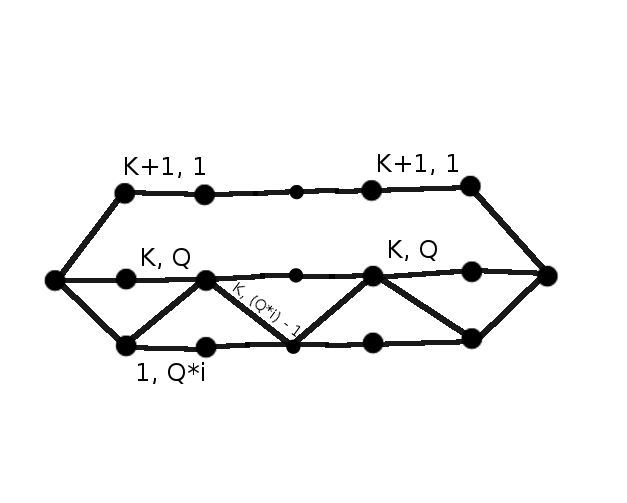
\includegraphics[width=\linewidth]{graficos/grafoFamiliaRompe2.png}
      \caption{\emph{3-caminos con puentes} $n=17$}\label{fig:familia-rompe2}
    \end{minipage}
  \end{center}
\end{figure}

Para esta familia de grafos se puede demostrar de manera muy similar a de la sección \ref{subsub:algoritmos-heuristicos-goloso-calidad.tex} que nuestro algoritmo goloso se queda con el camino $c$, que es el que está mas abajo.

Sin embargo, cuando corremos el algoritmo de busqueda local en un grafo de esta familia tomando como solución inicial la dada por nuestro algoritmo goloso, sí logra mejorarla. Esto es debido a que en este caso algunos nodos intermedios del camino $b$ y el camino $c$ sí están unidos por aristas. Debido a esto, partiendo de la solución inicial que nos da nuestro algoritmo goloso, que es el camino $c$, nuestro algoritmo de búsqueda local puede pasar de un camino a otro utilizando nuestra vecindad utilizando la operación Cambiar Nodo.

Lo que el algoritmo hace en el ejemplo es ir cambiando uno a uno los nodos intermedios del camino $c$ con su nodo correspondiente en el camino $b$. Vale aclarar que esto no se hace en cualquier orden ya inicialmente el algoritmo no puede cambiar cualquier nodo. Por ejemplo en el grafo de la Figura \ref{fig:familia-rompe2} el algoritmo puede, inicialmente, cambiar tanto el segundo nodo intermedio o el cuarto, pero no puede cambiar los otros, en este caso l algoritmo va a elegir cambiar el nodo que mejore más la solución. Supongamos que el algoritmo elige el segundo nodo, entonces en el segundo paso podrá cambiar el primer nodo intermedio o el cuarto.
